\tikzstyle{every picture}+=[remember picture]

\title{Connecting a website to native software with Node.JS}
\subtitle{}
\author{Victor Schubert <v@schu.be>}
\date{2020--02--04}

\frame{\titlepage}

\begin{frame}
	\frametitle{Our peculiar use case}

	\centering
	\Large
	\href{run:./init-patient.mkv}{Start video}
\end{frame}

\begin{frame}
	\frametitle{Overview}

	\centering
	\Large
	\begin{tikzpicture}[node distance=0.9,text height=.90em,text depth=.30em]
		\node (flar) [minimum width=11em,draw,rectangle] {Browser extension};
		\node (top) [rectangle,above=of flar]{~};
		\node (inet) [rectangle,above=of flar] {Doctolib webpage};
		\node (rora) [minimum width=11em,draw,rectangle,below=of flar] {Daemon};
		\node (psql) [minimum width=11em,draw,rectangle,below=of rora] {Specialized software};
		\draw (inet) edge[<->,>=stealth] node[anchor=west] {postMessage} (flar);
		\draw (flar) edge[<->,>=stealth] node(nmsg)[anchor=west] {Native messaging} (rora);
		\draw (rora) edge[<->,>=stealth] node[anchor=west] {AutoIT} (psql);
		\useasboundingbox (psql.south west) rectangle (top.north -| nmsg.east);
	\end{tikzpicture}

	% The talk will unfold from top to bottom.
\end{frame}

\begin{frame}
	\frametitle{Web extensions, a primer}

	\Large
	Web extensions are written in JS and composed of
	\begin{itemize}
		\item Content scripts running in tabs, with access to the DOM.
		\item Background scripts running separate from tabs.
		\item The manifest file which ties everything together.
	\end{itemize}
\end{frame}


\begin{frame}
	\frametitle{Native messaging?}

	\centering
	\LARGE
	\begin{tikzpicture}
		\node(extension) [rectangle,draw] { Extension };
		\path (extension.north west)
			+(-2ex,2ex) node(browser) [anchor=south west] { Browser };
		\path (browser.north west) coordinate(br-top-left);
		\path (extension.south east) +(2ex,-2ex) coordinate(br-bottom-right);
		\draw (browser.north west) rectangle (br-bottom-right);
		\path (br-bottom-right) +(12em,0em) coordinate(pr-bottom-right);
		\path (br-top-left) +(12em,0em) coordinate(pr-top-left);
		\draw (pr-top-left) rectangle (pr-bottom-right);
		\draw[line width=2pt,->,>=stealth] (br-bottom-right |- br-top-left) +(0em,-1em) coordinate(spawn-start) -- node[above]{\bfseries SPAWN!} (pr-top-left |- spawn-start);
		\node(process)  at ($(pr-top-left)!0.5!(pr-bottom-right)$)[anchor=center] {Process};
		\draw[line width=1pt,<->,>=stealth] (extension) -- node[below]{JSON} (extension -| pr-top-left);
	\end{tikzpicture}

	\vspace{1em}
	\large
	\texttt{npm install chrome-native-messaging}

	% \begin{itemize}
	% 	\item The browser spawns and manages a process.
	% 	\item It sends messages through the process’ standard input.
	% 	\item It receives messages from the process’ standard output.
	% 	\item Messages use a JSON-based protocol.
	% 	\item Not harder than \texttt{postMessage}.
	% \end{itemize}
\end{frame}

\begin{frame}
	\frametitle{So how is it all deployed?}

	\centering
	\Large
	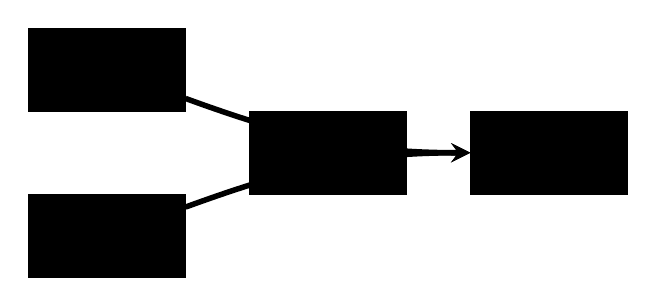
\begin{tikzpicture}[
			every node/.style={
				rectangle,
				draw,
				minimum width=5em,
				minimum height=3em,
				text width=5em,
				align=center,
				fill=black,
			},
			every edge/.style={
				>=stealth,
				draw,
				line width=2pt,
			}]
		\node(nodejs) at (-8em,3em)  {Node.JS interpreter};
		\node(mainjs) at (-8em,-3em) {JS script};
		\node(binary) at (8em,0em)   {Binary};
		\path (nodejs) edge[->,out=-20,in=180] (binary);
		\path (mainjs) edge[->,out=20,in=180] (binary);
		\node(pkg)    at (0em,0em)   {PKG};
	\end{tikzpicture}
\end{frame}

\begin{frame}
	\frametitle{Why use PKG?}

	\Large
	\begin{itemize}
		\item You don’t need to install Node.JS.
		\item You get cross-compilation for free.
		\item You can sign the binary.
	\end{itemize}
\end{frame}

% \begin{frame}
% 	\frametitle{The Zipper daemon}
% 
% 	// Schema showing messages flowing from the website through ZW and to
% 	ZD, and ZD doing the actions.
% 	% \begin{itemize}
% 	% 	\item Receives messages from the web extension.
% 	% 	\item Takes action upon receiving these messages.
% 	% 	\item Sends back messages with info and results.
% 	% 	\item Directly reads files.
% 	% 	\item Simulates user input on neighbouring software using AutoIT.
% 	% \end{itemize}
% \end{frame}

\begin{frame}[fragile]
	\frametitle{What’s AutoIT?}

	\Large
	\begin{verbatim}
WinActivate("Mozilla Firefox") ;
WinWaitActive("Mozilla Firefox") ;
Send("{HOME}") ;
Send("https://example.com") ;
Send("{ENTER}") ;
	\end{verbatim}
	% \begin{itemize}
	% 	\item Scripting language for GUI automation.
	% 	\item It is also a library!
	% 	\item But a DLL library.
	% 	\item There’s a basic binding, but not sufficient.
	% \end{itemize}
\end{frame}

\begin{frame}
	\frametitle{What’s a DLL again?}

	\Large
	\begin{itemize}
		\item A {\em Dynamic Link Library}.
		\item Contains code and data to be loaded and run by a program at runtime.
		\item That’s not very different from how CommonJS imports work.
	\end{itemize}
\end{frame}

% \begin{frame}
% 	\frametitle{DLLs aren’t too different from CommonJS modules actually}
% 
% 	\begin{columns}
% 	\begin{column}{0.5\textwidth}
% 		A DLL…
% 
% 		\begin{itemize}
% 			\item Has a symbol table.
% 			\item String keys in the symbol table point to functions and variables.
% 			\item Is loaded and cached/memoized by the OS.
% 		\end{itemize}
% 	\end{column}
% 	\begin{column}{0.5\textwidth}
% 		A CommonJS module…
% 
% 		\begin{itemize}
% 			\item Has an \texttt{exports} object.
% 			\item String keys in the \texttt{exports} object reference functions and variables.
% 			\item Is loaded and cached/memoized by Node.JS.
% 		\end{itemize}
% 	\end{column}
% 	\end{columns}
% \end{frame}

\definecolor{color1}{rgb}{1.000,0.604,0.447}
\definecolor{color2}{rgb}{0.447,0.898,1.000}

\begin{frame}
	\frametitle{CommonJS modules}

	\centering
	\Large
	\begin{tikzpicture}
		\node(const) at (0,0)    [anchor=south west] {
			\tt const data =
			\tikz[baseline]{\node(data-def)[inner sep=0,anchor=base]{\textcolor{color1}{42}};}
		};
		\node(function) at (0,-1) [anchor=south west] {
			\tt const foo =
			\tikz[baseline]{\node(foo-def)[inner sep=0,anchor=base]{\textcolor{color2}{(x) => x * data}};}
			};
		\node(exports) at (0,-2)  [anchor=south west] {
			\tt module.exports = \{
				\tikz[baseline]{\node(data-export)[inner sep=0,anchor=base]{\textcolor{color1}{data}};},
				\tikz[baseline]{\node(foo-export)[inner sep=0,anchor=base]{\textcolor{color2}{foo}};}
			\}
		};
		\begin{pgfonlayer}{background}
			\draw (data-export) edge[line width=1pt,->,shorten >=1ex, shorten <=1ex,out=90,in=0,>=stealth,color=color1] (data-def);
			\draw (foo-export)  edge[line width=1pt,->,shorten >=1ex, shorten <=1ex,out=90,in=270,>=stealth,color=color2] (foo-def);
		\end{pgfonlayer}
	\end{tikzpicture}
\end{frame}

\begin{frame}[fragile]
	\frametitle{Binary code}

	\LARGE
	\begin{Verbatim}
int data = 42;

int foo(int x) {
  return x * data;
}
	\end{Verbatim}
\end{frame}

\begin{frame}
	\frametitle{Binary code}

	\centering
	\LARGE
	\begin{tikzpicture}
		\node(l00) at (0,0)     {\Large\tt 70 6C 65 61 73 65 20 73};
		\node(l08) at (0,-2ex){\Large\tt 65 6E 64 20 68 65 6C 70};
		\node(l10) at (0,-4ex){\Large\tt 
			20 69 E2 80
			\tikz[baseline]{\node(data-hex)[inner sep=0,anchor=base]{\textcolor{color1}{2A 00 00 00}};}
		};
		\node(l18) at (0,-6ex){\Large\tt 99 6D 20 74 72 61 70 70};
		\node(l20) at (0,-8ex){\Large\tt \textcolor{color2}{65 64 20 69 6E 20 74 68}};
		\node(l28) at (0,-10ex){\Large\tt \textcolor{color2}{65 20 73 6F 66 74 77 61}};
		\node(l30) at (0,-12ex){\Large\tt 20 66 61 63 74 6F 72 79};
		\draw (l00.west |- 0,-14ex) -- (l00.east |- 0,-14ex);
		\node(l38) at (0,-16ex){\Large\tt \textcolor{color2}{f~ o~ o~ 00 20 00 00 00}};
		\node(l40) at (0,-18ex){\Large\tt \textcolor{color1}{d~ a~ t~ a~ 14 00 00 00}};

		\node at (l00.base west) [anchor=base east] {\small 00};
		\node at (l08.base west) [anchor=base east] {\small 08};
		\node at (l10.base west) [anchor=base east] {\small 10};
		\node at (l18.base west) [anchor=base east] {\small 18};
		\node at (l20.base west) [anchor=base east] {\small 20};
		\node at (l28.base west) [anchor=base east] {\small 28};
		\node at (l30.base west) [anchor=base east] {\small 30};
		\node at (l38.base west) [anchor=base east] {\small 38};
		\node at (l40.base west) [anchor=base east] {\small 40};

		\node at (l00.north east) [anchor=north west] {Data};
		\node at (l40.base east) [anchor=base west] {Symbol table};

		\begin{pgfonlayer}{background}
			\draw (l40) edge[line width=1pt,->,shorten >=1ex, shorten <=1ex,out=0,in=0,>=stealth,color=color1] (data-hex);
			\draw (l38) edge[line width=1pt,->,shorten >=1ex, shorten <=1ex,out=0,in=0,>=stealth,color=color2] (l20.south east);
		\end{pgfonlayer}
	\end{tikzpicture}

\end{frame}

\begin{frame}
	\frametitle{So how do we call that native function?}

	You can use either ffi or N-API. \vspace{1em}

	\begin{columns}[t]
		\begin{column}{0.5\textwidth}
			ffi…
			\begin{itemize}
				\item Is a Node.JS module.
				\item Requires explicit code to load the library.
				\item Requires all types to be rewritten in Javascript.
				\item Can call all function synchronously or asynchronously.
			\end{itemize}
		\end{column}
		\begin{column}{0.5\textwidth}
			N-API…
			\begin{itemize}
				\item Is an API for building C++ libraries called from JS.
				\item Requires you to write bindings in C++.
				\item Requires all types to be specified in C++.
				\item Requires extra work to offer asynchronous and synchronous
					variants of functions.
			\end{itemize}
		\end{column}
	\end{columns}
\end{frame}

\begin{frame}
	\frametitle{What when the DLL isn’t thread-safe?}

	\Large
	That’s a topic for an entire talk, or maybe a blog post, such as this one I wrote! \url{https://bit.do/thread-unsafe-ffi}
\end{frame}

\begin{frame}
	\frametitle{Want more?}

	\begin{center}
	\Large
	\begin{tabular}{>{\bfseries}ll}
		Name & Victor Schubert \\
		E-mail & v@schu.be \\
		Github & schubev \\
	\end{tabular}
		\vspace{1em}
	\newline
		\begin{tikzpicture}\draw (0,0) -- (6,0);\end{tikzpicture}
	\end{center}

	\large
	You’ll find more content from Doctolib there:
	\begin{itemize}
	\item Our blog at \url{https://medium.com/doctolib}
	\item A tech newsletter you can subscribe to at \url{https://bit.ly/DoctoTechLife}
	\item Job openings at \url{https://careers.doctolib.com}
	\item All the code and slides for this talk at \url{https://github.com/schubev/nodejs-berlin-ffi}
	\end{itemize}

\end{frame}
